\section{Arithmetic Operations}

\section*{Arithmetic Operations}
Flags (APSR = N, Z, C, V)\\
Instructions ending with with «S» allow flag modification

\begin{itemize}
  \item ADDS
  \item SUBS
  \item MOVS
  \item LSLS
\end{itemize}

\begin{center}
\begin{tabular}{|llll|}
\hline
Flag & Meaning & Action & Operands \\
\hline
Negative & MSB =1 & $\mathrm{N}=1$ & signed \\
Zero & Result $=0$ & $\mathrm{Z}=1$ & signed, unsigned \\
Carry & Carry & $\mathrm{C}=1$ & unsigned \\
Overflow & Overflow & $\mathrm{V}=1$ & signed \\
\hline
\end{tabular}
\end{center}

\section*{Overview}
\begin{itemize}
  \item ADD / ADDS
  \item ADCS Addition with Carry
  \item ADR Address to Register
  \item SUB / SUBS
  \item SBCS
  \item RSBS
  \item MULS
\end{itemize}

Subtraction\\
Subtraction with carry (borrow)\\
Reverse Subtract (negative)\\
Multiplication\\
$A+B$\\
$A+B+c$\\
$P C+A$\\
$A-B$\\
$A-B-!c$\\
$-1 \cdot A$\\
$A \cdot B$

Multi-Word Addition with ADCS\\
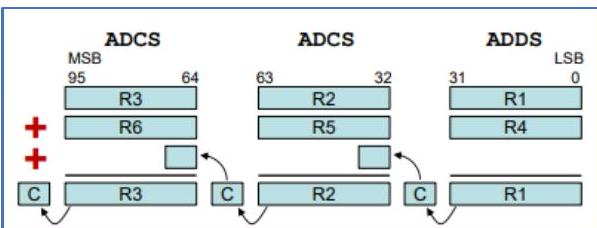
\includegraphics[width=\linewidth]{images/2024_12_29_79e6b22f503fb7b4f718g-04}

\begin{center}
\begin{tabular}{|c|c|c|c|}
\hline
ADDS & R1, & R1, & R4 \\
\hline
ADCS & R2, & R2, & R5 \\
\hline
ADCS & R3, & R3, & R6 \\
\hline
\end{tabular}
\end{center}

Multi-Word Subtraction with SBCS\\
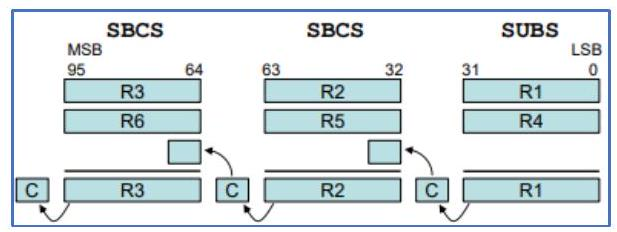
\includegraphics[width=\linewidth]{images/2024_12_29_79e6b22f503fb7b4f718g-04(1)}

\begin{center}
\begin{tabular}{|c|c|c|c|}
\hline
SUBS & R1, & R1, & R4 \\
\hline
SBCS & R2, & R2, & R5 \\
\hline
SBCS & R3, & R3, & R6 \\
\hline
\end{tabular}
\end{center}

\section*{Negative Number}
\begin{itemize}
  \item 2' Complement $\quad A=!A+1$
\end{itemize}

\section*{Carry and Overflow}
unsigned

\begin{itemize}
  \item Addition $\rightarrow \quad \mathrm{C}=1 \rightarrow$ carry result too large for available bits
  \item Subtraction $\rightarrow \mathrm{C}=0 \rightarrow$ borrow result less than zero $\rightarrow$ no negative numbers\\
signed
  \item Addition $\rightarrow \quad$ potential overflow in case of operands with equal signs
  \item Subtraction $\rightarrow$ potential overflow in case of operands with opposite signs
\end{itemize}

\section*{Addition and Subtraction}
\begin{itemize}
  \item Addition $\quad \mathrm{C}=1 \rightarrow$ Carry
\end{itemize}

\begin{center}
\begin{tabular}{|rrrrr|}
\hline
1 & 1 & 0 & 1 & $13 d$ \\
0 & 1 & 1 & 1 & $7 d$ \\
1 & 1 & 1 & 1 &  \\
1 &  &  &  &  \\
1 & 0 & 1 & 0 & 0 \\
\end{tabular}
\end{center}

\begin{itemize}
  \item Subtraction $\quad \mathrm{C}=0 \rightarrow$ Borrow sign\\
$6 d-14 d=0110 b-1110 b=0110 b+0010 b$
\end{itemize}

$$
\begin{array}{llllll}
0 & 1 & 1 & 0 & 6 d \\
0 & 0 & 1 & 0 & 2 d=\operatorname{TC}(14 d)
\end{array}
$$

0100\\
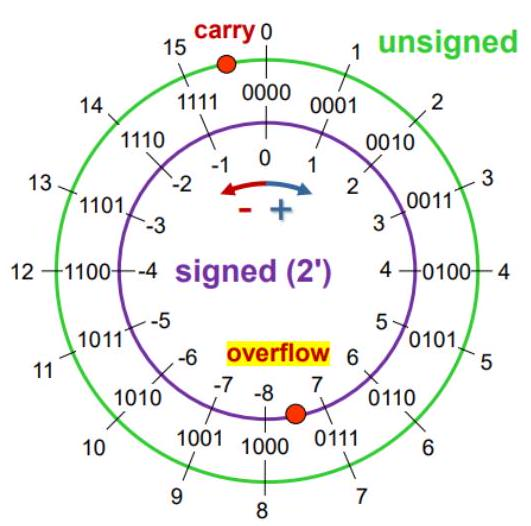
\includegraphics[width=\linewidth]{images/2024_12_29_79e6b22f503fb7b4f718g-04(2)}
